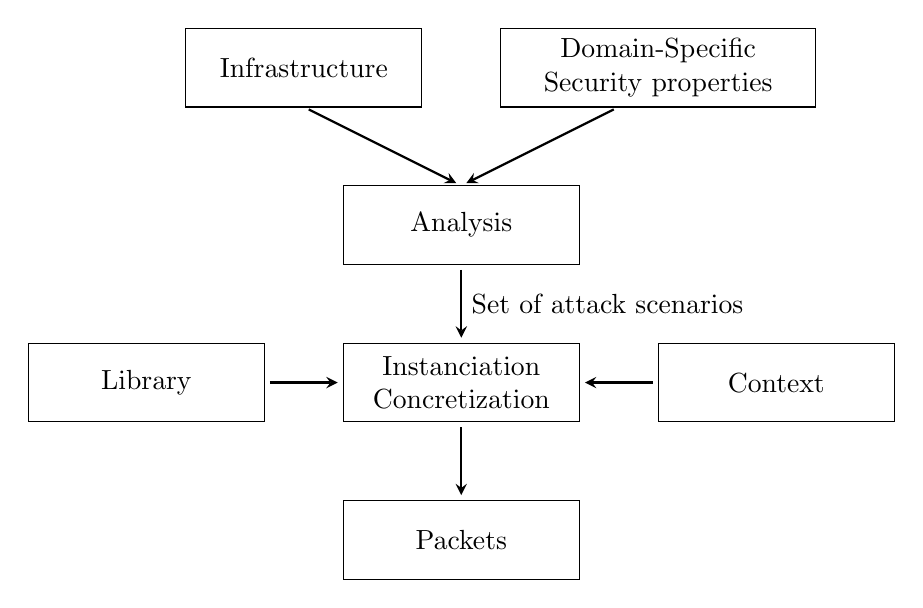
\begin{tikzpicture}[
        arrow/.style={thick,->,shorten >=2pt,shorten <=2pt,>=stealth},
    ]
    \draw (2,6) rectangle (5,7) node [pos=.5] {Infrastructure};
    \draw (6,6) rectangle (10,7) node [pos=.5,align=center] {Domain-Specific\\Security properties};

    \draw (4,4) rectangle (7,5) node [pos=.5] {Analysis};

    \draw (0,2) rectangle (3,3) node [pos=.5] {Library};
    \draw (4,0) rectangle (7,1) node [pos=.5] {Packets};
    \draw (8,2) rectangle (11,3) node [pos=.5] {Context};

    \draw (4,2) rectangle (7,3) node [align=center,pos=.5] {Instanciation\\Concretization};

    \draw[arrow] (3.5,6) -- (5.5,5); % Archi --> Analyses
    \draw[arrow] (7.5,6) -- (5.5,5); % Props --> Analyses
    \draw[arrow] (5.5,4) -- (5.5,3) node [pos=.5,right] {Set of attack scenarios}; % Analyses --> Inst
    \draw[arrow] (3,2.5) -- (4,2.5); % Biblio --> Inst
    \draw[arrow] (8,2.5) -- (7,2.5); % Context--> Inst
    \draw[arrow] (5.5,2) -- (5.5,1); % Inst --> Packets
\end{tikzpicture}
